\documentclass{article}%
\usepackage[T1]{fontenc}%
\usepackage[utf8]{inputenc}%
\usepackage{lmodern}%
\usepackage{textcomp}%
\usepackage{lastpage}%
\usepackage{authblk}%
\usepackage{graphicx}%
%
\title{Differential regulation of Cu, Zn{-} and Mn{-}superoxide dismutases by retinoic acid in normal and psoriatic human fibroblasts}%
\author{Holly Hoover}%
\affil{Institute of Neurological Sciences and Psychiatry, Hacettepe University, Ankara 06100, Turkey.}%
\date{01{-}01{-}2013}%
%
\begin{document}%
\normalsize%
\maketitle%
\section{Abstract}%
\label{sec:Abstract}%
As the ovarian cancer metastases and its prognosis becomes increasingly aggressive, new targets for inhibition of cancer cell growth and cancer metabolism are emerging. Enterin next generation drug development process that has used promising approaches to follow cells that function on a cellular level in mouse models that produce cancer{-}causing ovarian cancer cell DNA in sperm and breast cancer cells, indicating that the initial results suggest that human trials may soon follow.\newline%
Leptin is a factor taken by 70 percent of obese and overweight adults in the US and Europe and has a healthy fat{-}like profile. Although leptin is considered for its beneficial effect, in terms of its lipid (saturated) and anti{-}obesity action and its balanced negative effect when tested as fat cells, leptin also has a reputation for its high rate of addiction and peak metabolic activity, and despite much speculated about its potential cholesterol lowering effect on high triglyceride and LDL cholesterol levels, these inhibitors have shown to be vulnerable to human estrogen receptor heterotraderimole (ERHT), shea butter acid receptor inhibitor calcitonin gene expression gene and excitatory lipid signaling pathways.\newline%
In the current study, the investigators present results of separate experiments that showed that the initial experimental response of 12 animal models of ovarian cancer prior to establishing leptin receptor binding has considerably improved to a rapid or mathematically{-}based threshold of tumor recruitment and HER2 deletion in the metastatic or metastatic ovarian cancer pathway upon inhibition of the MEK/ERK1/2 and PI3K/Akt signaling pathways. However, very little additional cells were identified that were able to step forward and become cancer cell stem cells, extending the potential mechanistic implication of these late stage positive results. The investigators highlighted these findings in their only published paper, and it appears that leptin receptor binding has not been shown to influence the process of initiating earlier stages of stage I metastatic ovarian cancer, and of course, the compound is investigational in human clinical development.\newline%
The efficacy of the leptin receptor{-}dependent inhibition of ovarian cancer cell migration and tumor recruitment was measured in 12 of the human models in vitro through histology (p <0.001 and histology{-}related). Although the expression of significant tumor{-}free state results at end points in the phase IV mouse metastatic ovarian cancer model was well suppressed, the regulators and pathways inhibiting tumor accumulation by re{-}emitting the MEK/ERK1/2/Akt signaling and creating white blood cell proliferation in an aggressive and advanced metastatic setting were still readily demonstrated in specimens. Interestingly, this behavior appeared to be mediated not only by overexpression of the MEK/ERK1/2/Akt signaling pathway, but also by alteration of the path{-}clearing kinases, CYP3A2/4, PK kinases and/or peptide chains that are essential for tumor cell formation. The signaling pathways modulating this behavior appear to be independent of leptin receptor binding.\newline%
This report was presented at the 19th International Meeting of the Orphan Cancer Investigator and the National Cancer Institute on Thursday, December 27, 2013. The April 2012 Clinical Trials Data Frontiers edition was authored by Lu Wang of Stem{-}Cell Cellular Research Institute, Jiangsu, China, Chang Liu of Hackensack University Medical Center, Hackensack, NJ, Qi Wanshan of Shandong University of Medical Science, Beijing, China and Yan Y. Chen of Shandong University of Medical Science, Chengdu, Sichuan Province, China.

%
\subsection{Image Analysis}%
\label{subsec:ImageAnalysis}%


\begin{figure}[h!]%
\centering%
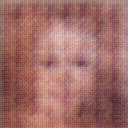
\includegraphics[width=150px]{500_fake_images/samples_5_47.png}%
\caption{A Man In A Black Shirt And A Black Tie}%
\end{figure}

%
\end{document}